\section{Wyniki}

\textcolor{red}{Tu wypadałoby jakiś komentarz też. Wyznaczone wartości i porównanie z teoretycznymi.}

Rysunek \ref{img:mass} przedstawia uzyskany histogram masy mezonu K$^0_\text{s}$.

\begin{figure}[H]
	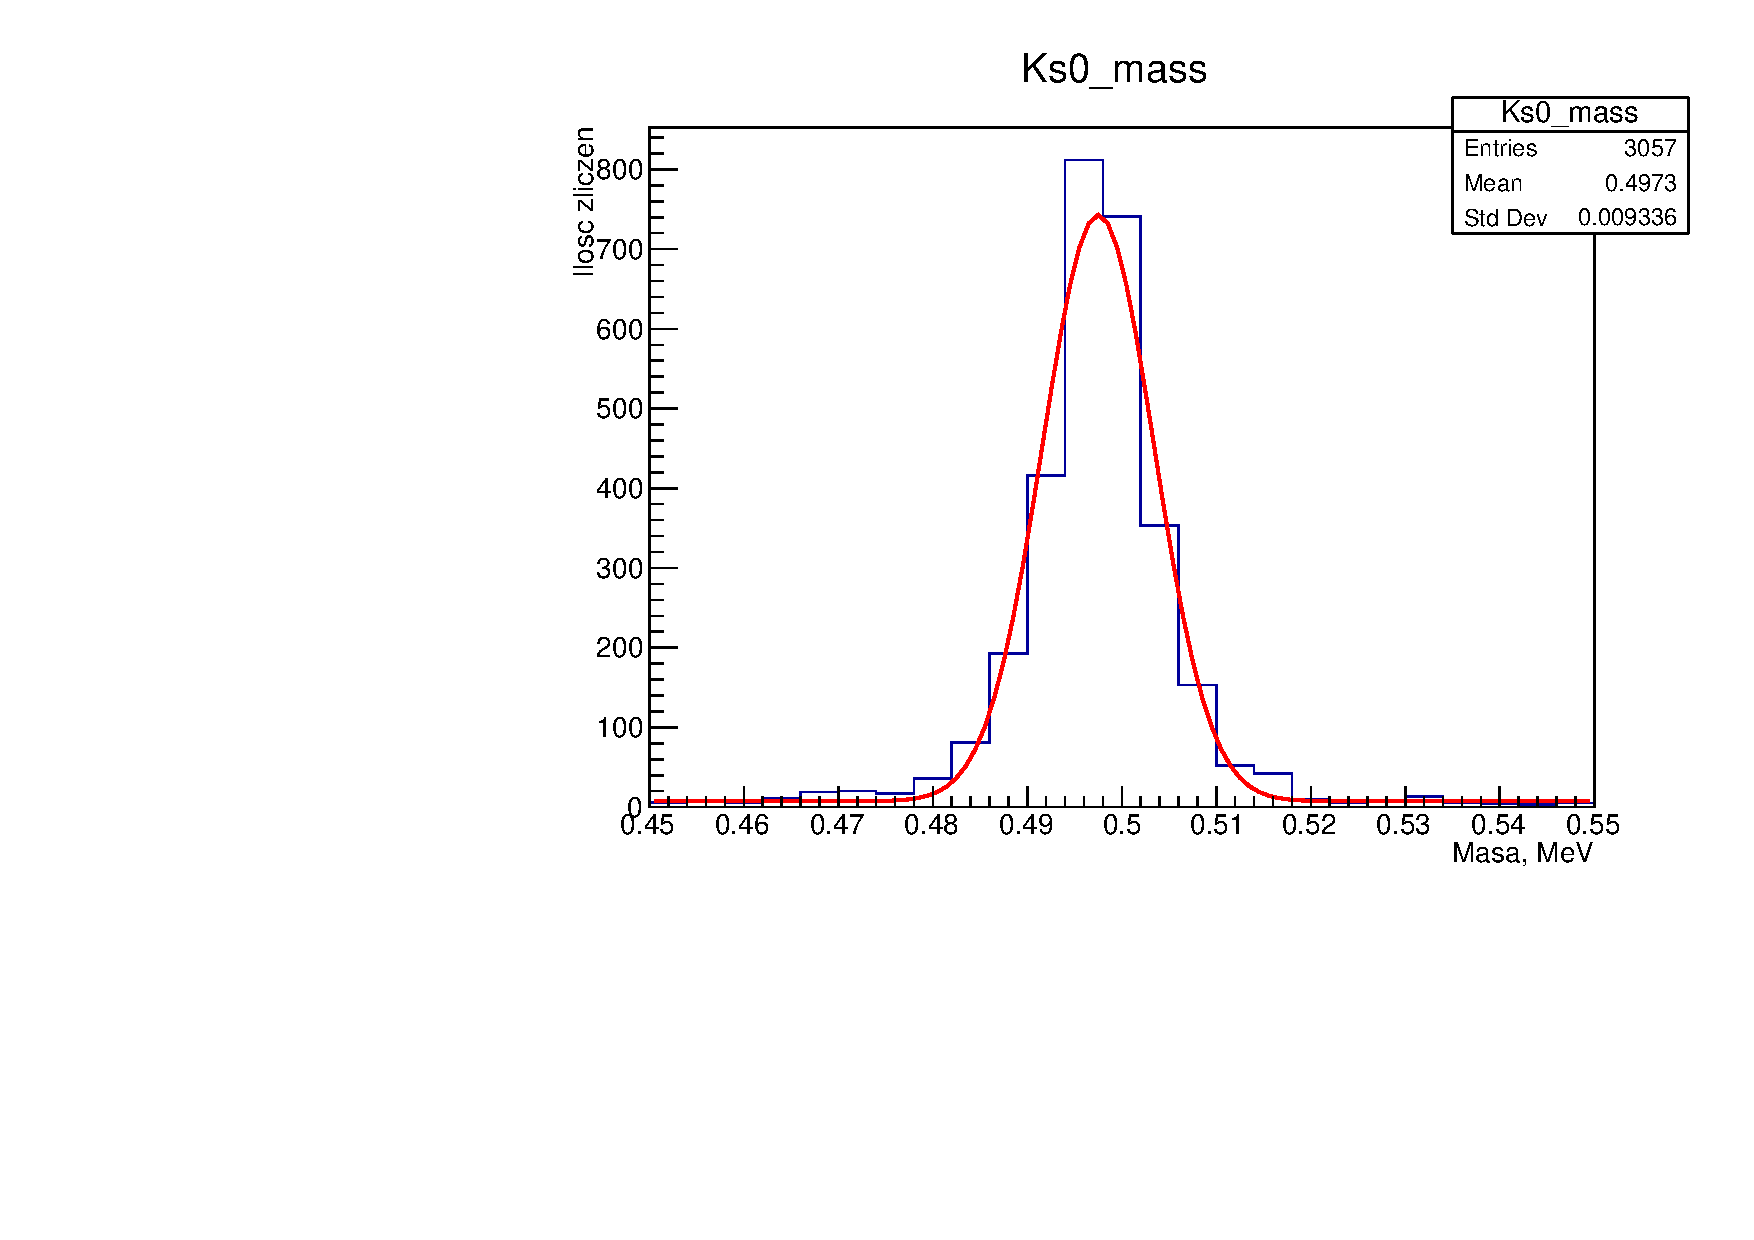
\includegraphics[width=\textwidth]{ceiio/ks0mass}
	\caption{Otrzymany rozkład masy z dopasowaną krzywą Gaussa}
	\label{img:mass}
\end{figure}

Do histogramu dopasowano krzywą Gaussa z dodanym stałym tłem. Uzyskano wartość średnią $497.3\ \mega\electronvolt$, oddaloną od wartości tablicowej $497.6\ \mega\electronvolt$ o mniej niż wartość odchylenia standardowego.

Rysunek \ref{img:tau} przedstawia uzyskany histogram czasu życia mezonu K$^0_\text{s}$.

\begin{figure}[H]
	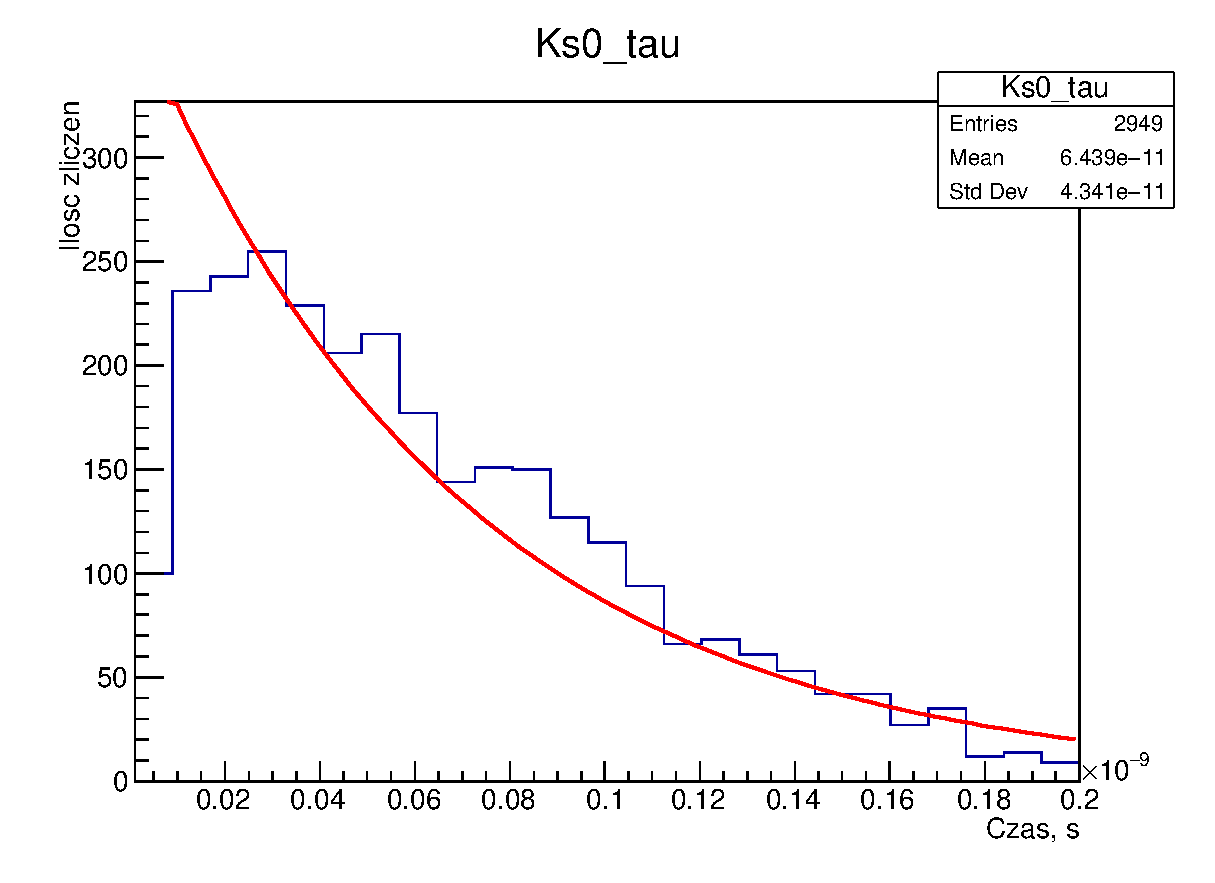
\includegraphics[width=\textwidth]{ceiio/ks0tau}
	\caption{Otrzymany rozkład czasu życia z dopasowaną eksponentą}
	\label{img:tau}
\end{figure}

Wartość tablicowa czasu życia zawiera się w uzyskanym wyniku, jednak otrzymana dokładność jest bardzo niska, ponieważ odchylenie standardowe $4.34 \cdot 10^{-11}\ \second$ jest tego samego rzędu co wartość średnia $6.44 \cdot 10^{-11}\ \second$.